% ----------------------------------------------------------
\chapter{Desenvolvimento do Projeto}
% ----------------------------------------------------------

Depois das definições apresentadas e da escolha de componentes apresentada na seção anterior, foi possível elaborar um esquemático elétrico, que mostra os circuitos relevantes do OBDH. Nesse capítulo, discutir-se-á circuitos específicos mais relevantes do projeto, usando o esquemático pronto, que se encontra no Apêndice A. O \textit{software} utilizado para elaboração desse esquemático foi o Altium Designer (versão 24.4.1).

\section{Conversores de Potência}

Partindo do princípio que o módulo EPS da terceira geração de módulos do SpaceLab será capaz de fornecer 3,3 V para o OBDH, foi proposta uma cascata de potência descrita na Figura \ref{fig:power}. Nela, são suprimidos os circuitos de proteção que serão descritos posteriormente.

\begin{figure}[H]
    \centering
    \caption{Cascata de potência proposta.}
    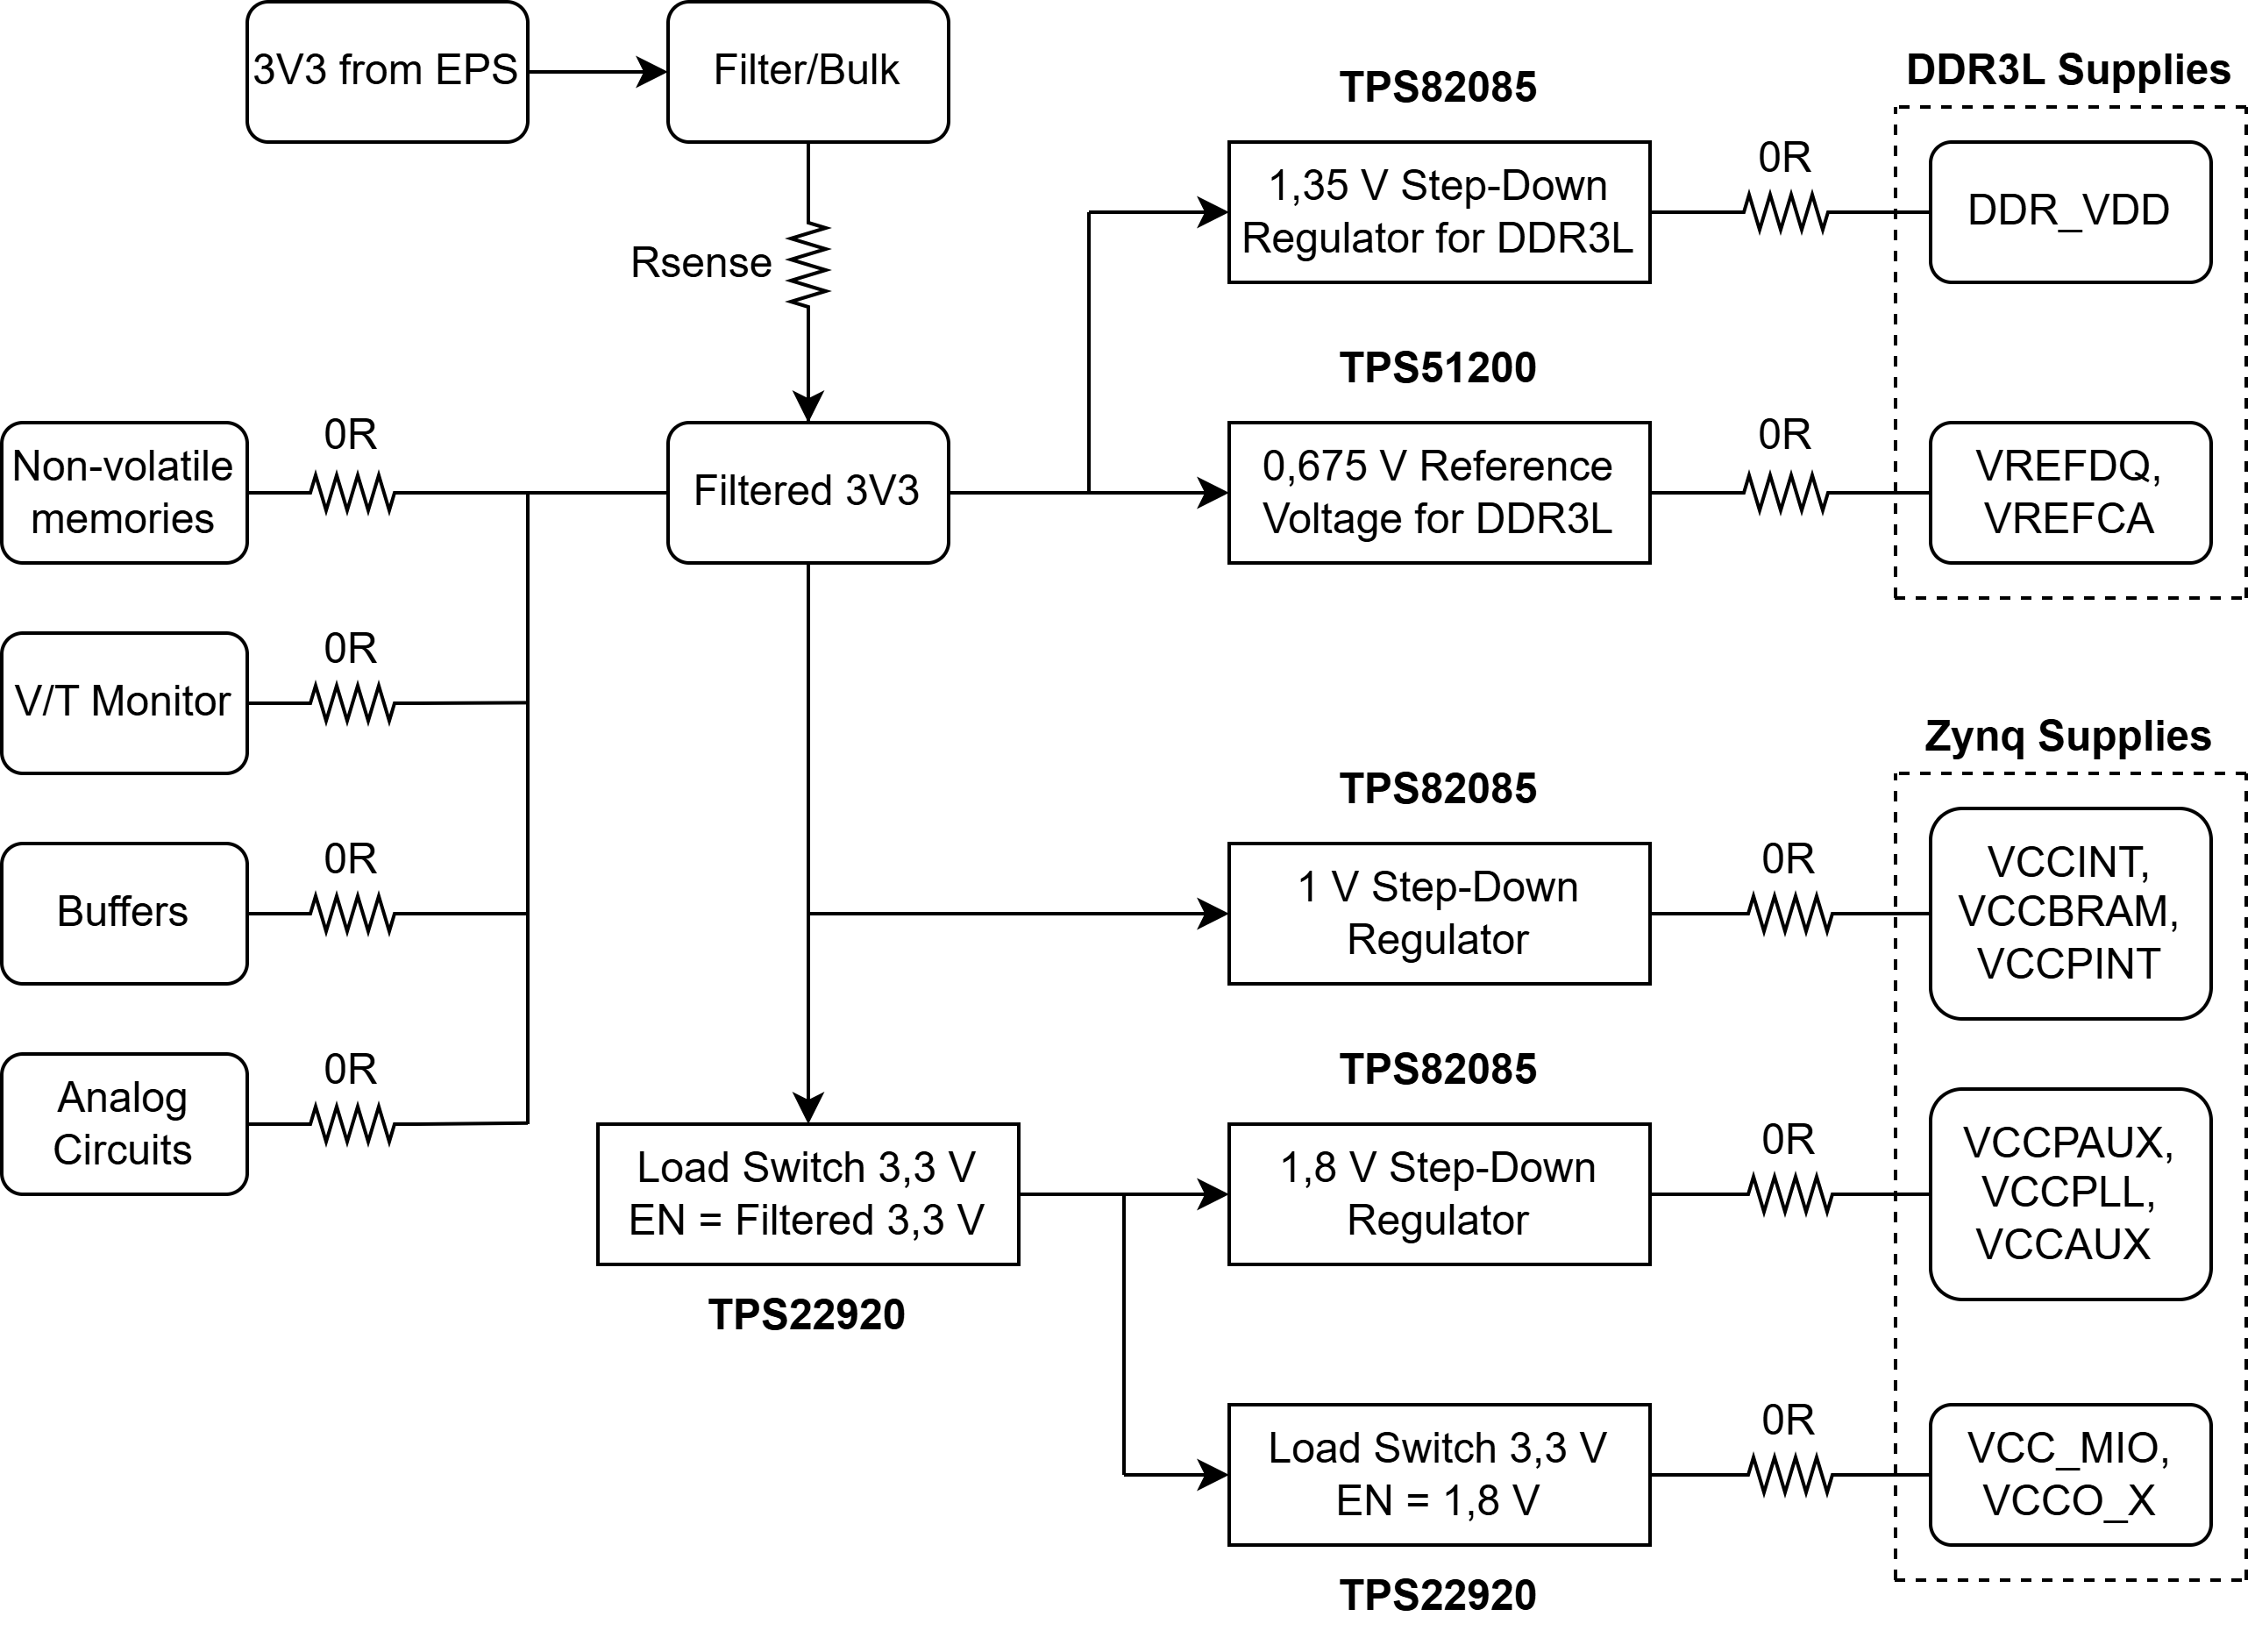
\includegraphics[scale=0.8]{images/Power_system.png}
    \label{fig:power}
    \fonte{Elaboração própria.}
\end{figure}

\subsection{Filtro de Entrada}

Costumeiramente, a entrada de tensão de uma placa robusta deve ser filtrada, principalmente devido às flutuações do ruído conduzido de outros subsistemas do satélite, caracterizando o fenômeno de Interferência Eletromagnética (EMI), esquematizado na Figura \ref{fig:emi}.

\begin{figure}[H]
    \centering
    \caption{Interferência com ruído conduzido.}
    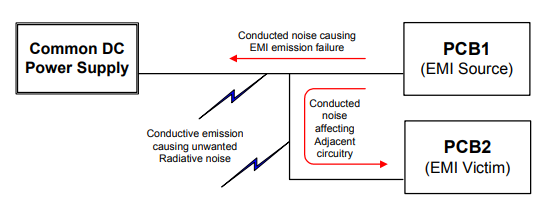
\includegraphics[scale=1]{images/EMI noise.png}
    \label{fig:emi}
    \fonte{SOH et al., 2010.}
\end{figure}

Além disso, também foi necessária a inclusão de um diodo Zener em paralelo à entrada, servindo como um elemento extra de proteção contra perturbações e transientes (CADENCE, 2023). Outra característica explorada foi a colocação de capacitores em paralelo, a fim de reduzir sua resistência em série equivalente (ESR) e sua indutância série (SARJEANT, 1990).  O filtro proposto está disposto na Figura \ref{fig:FILTRO}.  Além disso, sua magnitude e fase simuladas estão dispostas na Figura \ref{fig:filtrof}, utilizando o software LTSPICE XVII.

\begin{figure}[H]
    \centering
    \caption{Filtro proposto.}
    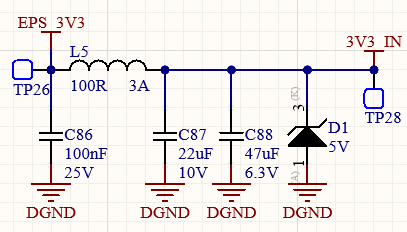
\includegraphics[scale=1]{images/FILTRO.png}
    \label{fig:FILTRO}
    \fonte{Elaboração própria.}
\end{figure}

\begin{figure}[H]
    \centering
    \caption{Simulação de magnitude e fase em função da frequência para o filtro proposto.}
    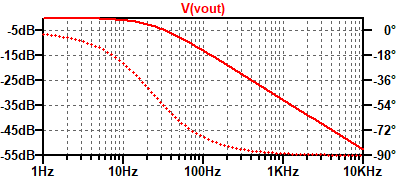
\includegraphics[scale=1]{images/filtrof.png}
    \label{fig:filtrof}
    \fonte{Elaboração própria.}
\end{figure}

\subsection{Cascata de potência}

Devido à escolha do SoC e da memória DDR3, foi necessária a definição de uma cascata de potência, levando-se em consideração os requisitos de (UG585, 2023), que descreve o sequenciamento das tensões para o menor consumo de potência e para garantir a integridade do fusível interno do SoC. Dessa forma, como pode-se ver na Figura \ref{fig:power}, são usados os denominados \textit{load switches}, a fim de garantir o sequenciamento descrito e garantir uma proteção efetiva contra sobrecorrente (MAK, 2018). 

O primeiro regulador, que gera a tensão de 1 V, apresentado na Figura \ref{fig:1vsupp}, é o primeiro da cascata. Seu divisor de tensão de saída foi calculado conforme (TPS82085, 2019):

\begin{equation}
	V_{out} = 0,8 * (1 + R_1/R_2) = 0,8 * (1+ 37,4k/150k) = 0,999 V
\end{equation} 

\begin{figure}[H]
    \centering
    \caption{Regulador de tensão de 1 V.}
    \includegraphics[scale=0.8]{images/1vsupp.png}
    \label{fig:1vsupp}
    \fonte{Elaboração própria com base no circuito apresentado pelo fabricante.}
\end{figure}

Também foi possível montar seu circuito de proteção de sobrecorrente, disposto na Figura \ref{fig:1vocp}. Seu resistor de entrada, que escolhe o limiar de corrente permitido, foi caculado conforme (LTC4361, 2018), considerando uma corrente 20\% superior à máxima calculada (na Tabela \ref{tab:estpow}):

\begin{equation}
	R_{sense} = 50 mV / I_{max} =50 / 0,94 = 53 m\Omega
\end{equation} 

\begin{figure}[H]
    \centering
    \caption{Proteção contra \textit{latch-up} para a tensão de 1 V.}
    \includegraphics[scale=1]{images/1vocp.png}
    \label{fig:1vocp}
    \fonte{Elaboração própria com base no circuito apresentado pelo fabricante.}
\end{figure}

Depois disso, para seguir com o sequenciamento requerido pelo SoC, precisa-se de um circuito de chaveamento de carga, apresentado na Figura \ref{fig:sw1}. Seu circuito é baseado no sugerido por (TPS22920, 2016), com sua ativação o sendo realizada pela própria tensão de 3,3 V.

\begin{figure}[H]
    \centering
    \caption{Circuito de \textit{Load switch} para a tensão de 1,8 V.}
    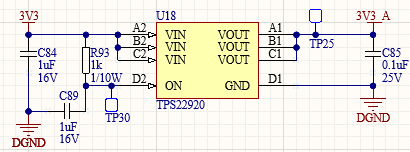
\includegraphics[scale=1]{images/sw1.png}
    \label{fig:sw1}
    \fonte{Elaboração própria com base no circuito apresentado pelo fabricante.}
\end{figure}

Analogamente, para a tensão de 1,8 V, são necessários ambos um conversor e um circuito de proteção. Estes estão dispostos respectivamente nas Figuras \ref{fig:1v8supp} e \ref{fig:1v8ocp} a seguir, conjuntamente com suas equações (3) e (4) para obtenção das resistências requeridas, usando a mesma margem de 20\% de corrente máxima. 

\begin{equation}
	V_{out} = 0,8 * (1 + R_1/R_2) = 0,8 * (1+ 110k/88,7k) = 1,792 V
\end{equation} 

\begin{figure}[H]
    \centering
    \caption{Regulador de tensão de 1,8 V.}
    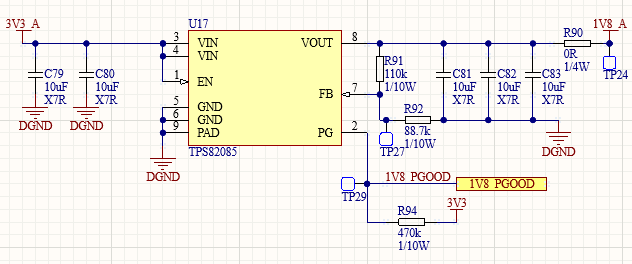
\includegraphics[scale=0.8]{images/1v8supp.png}
    \label{fig:1v8supp}
    \fonte{Elaboração própria com base no circuito apresentado pelo fabricante.}
\end{figure}

\begin{equation}
	R_{sense} = 50 mV / I_{max} =50 / 0,38 = 131 m\Omega
\end{equation} 

\begin{figure}[H]
    \centering
    \caption{Proteção contra \textit{latch-up} para a tensão de 1,8 V.}
    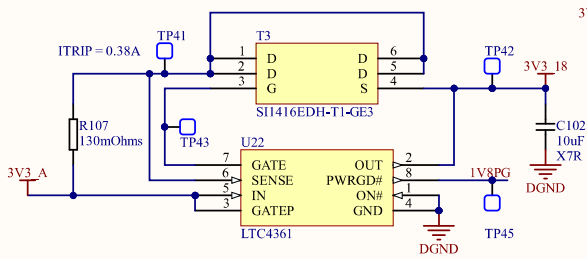
\includegraphics[scale=1]{images/1v8ocp.png}
    \label{fig:1v8ocp}
    \fonte{Elaboração própria com base no circuito apresentado pelo fabricante.}
\end{figure}

Por fim, para ligar a tensão de 3,3 V fornecida para o SoC, é necessário um último circuito de chaveamento, dessa vez com sua ativação realizada pela tensão de 1,8 V, como mostra a Figura \ref{fig:sw2}. Na Figura \ref{fig:3v3ocp} se encontra o circuito de proteção proposto.

\begin{figure}[H]
    \centering
    \caption{Circuito de \textit{Load switch} para a tensão de 3,3 V do SoC.}
    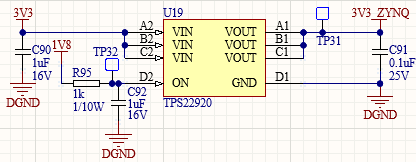
\includegraphics[scale=0.8]{images/sw2.png}
    \label{fig:sw2}
    \fonte{Elaboração própria com base no circuito apresentado pelo fabricante.}
\end{figure}

\begin{equation}
	R_{sense} = 50 mV / I_{max} =50 / 0,5 = 100 m\Omega
\end{equation} 

\begin{figure}[H]
    \centering
    \caption{Proteção contra \textit{latch-up} para a tensão de 3,3 V para o SoC.}
    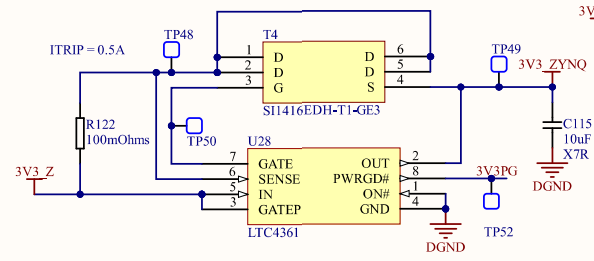
\includegraphics[scale=0.8]{images/3v3ocp.png}
    \label{fig:3v3ocp}
    \fonte{Elaboração própria com base no circuito apresentado pelo fabricante.}
\end{figure}

Paralelamente, para a memória DDR3L, são necessários um conversor para a alimentação, de 1,35 V, e um conversor para a tensão de referência e de terminação. Esses circuitos estão dispostos respectivamente nas Figuras \ref{fig:1v35supp} e \ref{fig:1v35ref}. No caso da tensão de alimentação de 1,35 V, também foi colocado um circuito de proteção, como mostra a Figura \ref{fig:1v35ocp}.

\begin{equation}
	V_{out} = 0,8 * (1 + R_1/R_2) = 0,8 * (1+ 47k/68k) = 1,353 V
\end{equation} 

\begin{figure}[H]
    \centering
    \caption{Regulador de tensão de 1,35 V.}
    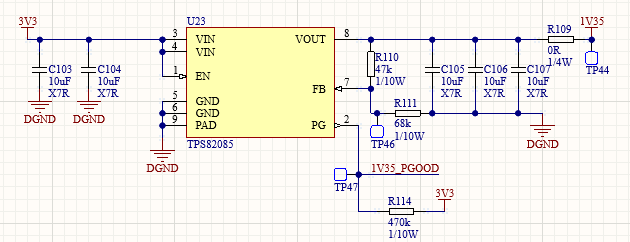
\includegraphics[scale=0.8]{images/1v35supp.png}
    \label{fig:1v35supp}
    \fonte{Elaboração própria com base no circuito apresentado pelo fabricante.}
\end{figure}

\begin{equation}
	R_{sense} = 50 mV / I_{max} =50 / 0,13 = 384 m\Omega
\end{equation} 

\begin{figure}[H]
    \centering
    \caption{Proteção contra \textit{latch-up} para a tensão de 1,35 V.}
    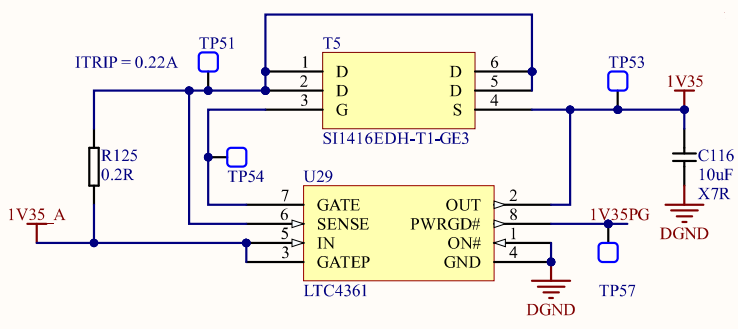
\includegraphics[scale=0.8]{images/1v35ocp.png}
    \label{fig:1v35ocp}
    \fonte{Elaboração própria com base no circuito apresentado pelo fabricante.}
\end{figure}


\begin{figure}[H]
    \centering
    \caption{Regulador de tensão de referência e terminação para a memória DDR3L.}
    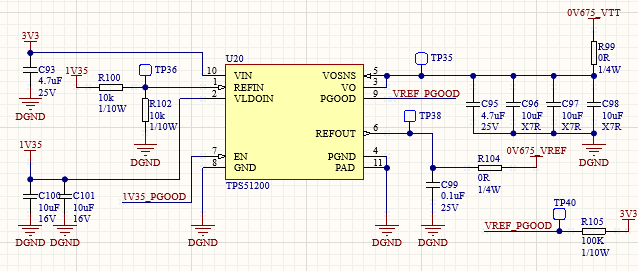
\includegraphics[scale=0.8]{images/refsupp.png}
    \label{fig:1v35ref}
    \fonte{Elaboração própria com base no circuito apresentado pelo fabricante.}
\end{figure}

Finalmente, para os outros circuitos conectados ao barramento de alimentação de 3,3 V, foi colocado mais uma proteção contra o efeito de \textit{latch-up}, disposta na Figura \ref{fig:3v3gocp}.

\begin{equation}
	R_{sense} = 50 mV / I_{max} =50 / 2,72 = 18,4 m\Omega
\end{equation} 

\begin{figure}[H]
    \centering
    \caption{Proteção contra \textit{latch-up} para a tensão de 3,3 V para outros circuitos do OBDH.}
    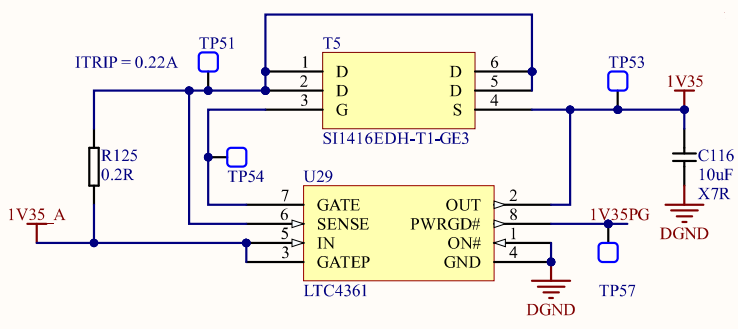
\includegraphics[scale=0.8]{images/1v35ocp.png}
    \label{fig:3v3gocp}
    \fonte{Elaboração própria com base no circuito apresentado pelo fabricante.}
\end{figure}

\section{SoC}

No caso do SoC Zynq 7030, temos no total seis blocos operacionais, que incluem o funcionamento do PL e do PS, bem como as configurações e o bloco dedicado ao controlador da memória DDR (UG585, 2023). A seguir, estão dispostas as descrições funcionais e circuitos necessários para o funcionamento correto desse SoC, separados por cada um dos blocos citados.

\subsection{Bloco de Configuração}

O banco zero do SoC é o responsável por algumas opções e sinais de configuração. Abaixo, na Tabela \ref{tab:config}, se encontra a descrição funcional de cada pino desse banco, esquematizado na Figura \ref{fig:config}. Esse esquemático, bem como seus resistores de \textit{pull-up} (Figura \ref{fig:pullupconfig}), foram baseados na documentação técnica fornecida pela Xilinx (UG865, 2023) (UG470, 2023) (UG933, 2019) (DS191, 2018).


\begin{table}[H]
	\ABNTEXfontereduzida
	\caption{\label{tab:config}Descrição funcional dos pinos de configuração.}
	%\begin{tabular}{@{}p{2cm}p{2cm}p{2cm}p{2cm}p{2cm}p{2cm}p{3cm}@{}}
    \centering
    \begin{tabular}{@{} >{\centering}p{4cm} >{\centering}p{8cm} @{}}
    
		\toprule
		\textbf{Nome} & \textbf{Função} \tabularnewline 
        \midrule
         DXN e DXP & Terminais do diodo interno para medição de temperatura. \tabularnewline
         \midrule

         VREFP e VREFN & Tensões de referência do conversor analógico digital (XADC) do SoC. \tabularnewline

       \midrule
        VP e VN & Entrada extra do XADC. \tabularnewline

       \midrule
        VCCBAT & Não utilizada. Fonte da bateria. \tabularnewline

       \midrule
        TCK, TMS, TDI e TDO & Sinais da interface JTAG.  \tabularnewline

       \midrule
        INIT\_B & Indica inicialização da memória interna de configuração. \tabularnewline

       \midrule
       PROGRAM\_B & Reset assíncrono da lógica de configuração. \tabularnewline

       \midrule
        CFGBVS & Pino que seleciona o tipo de IO do banco 0. \tabularnewline

       \midrule
        DONE & Indica que a configuração foi terminada e feita corretamente. \tabularnewline

       \midrule
        VCCADC e GNDADC & Alimentação do XADC. \tabularnewline

       \midrule
        RSVDVCC e RSVDGND & Pinos de alimentação reservados. \tabularnewline

        \bottomrule
	\end{tabular}
	\fonte{Elaboração própria com base na documentação técnica do fabricante.}
\end{table}

\begin{figure}[H]
    \centering
    \caption{Banco de configuração do SoC.}
    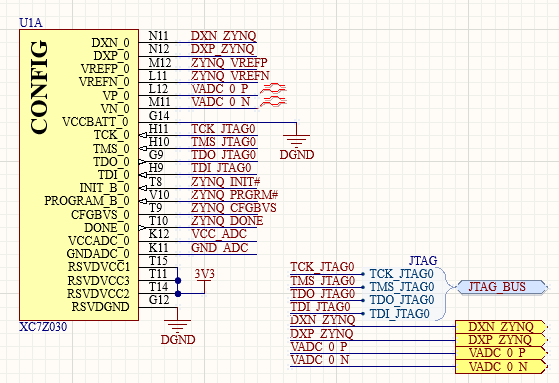
\includegraphics[scale=0.8]{images/zynqconfig.png}
    \label{fig:config}
    \fonte{Elaboração própria com base no circuito apresentado pelo fabricante.}
\end{figure}

\begin{figure}[H]
    \centering
    \caption{Resistores de \textit{pull-up} necessários.}
    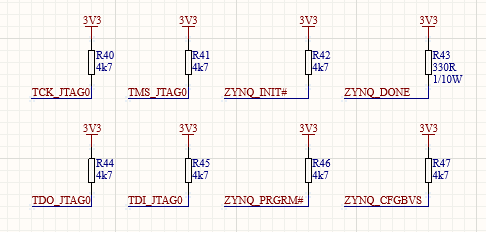
\includegraphics[scale=0.8]{images/pullupconfig.png}
    \label{fig:pullupconfig}
    \fonte{Elaboração própria com base no circuito apresentado pelo fabricante.}
\end{figure}

Além disso, para a alimentação do XADC (\textit{Xilinx Analog to Digital Converter}), foi necessário um circuito de filtragem, disposto na Figura \ref{fig:xadcfilter}, como requerido por (UG480, 2022).

\begin{figure}[H]
    \centering
    \caption{Filtro da alimentação analógica do SoC.}
    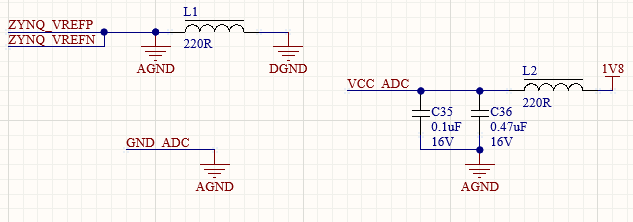
\includegraphics[scale=0.8]{images/xadcfilter.png}
    \label{fig:xadcfilter}
    \fonte{Elaboração própria com base no circuito apresentado pelo fabricante.}
\end{figure}


\subsection{Blocos do PS}

No caso do sistema de processamento (PS), existem três bancos principais. O primeiro, denominado MIO (\textit{Multiplexed In-Out}), é onde se encontram os controladores das interfaces de comunicação, bem como a entrada de relógio e a escolha do \textit{boot}. No caso desse projeto, foi decidido que o SoC poderá inicializar de duas formas, sendo a primeira pela interface JTAG e a segunda pela memória Flash NOR (QSPI), escolhidos pelos resistores R48 e R51. O banco MIO e seus modos de inicialização estão dispostos nas Figuras \ref{fig:psmio} e \ref{fig:boot}.

\begin{figure}[H]
    \centering
    \caption{Banco MIO do SoC com suas respectivas entradas e saídas.}
    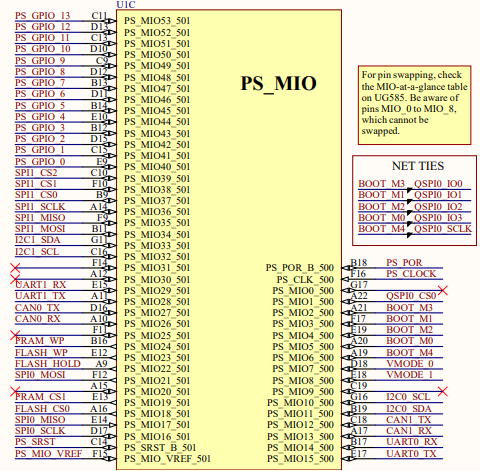
\includegraphics[scale=0.8]{images/psmio.png}
    \label{fig:psmio}
    \fonte{Elaboração própria com base na Tabela MIO-at-a-glance (UG585, 2023).}
\end{figure}

\begin{figure}[H]
    \centering
    \caption{Modos de inicialização do SoC.}
    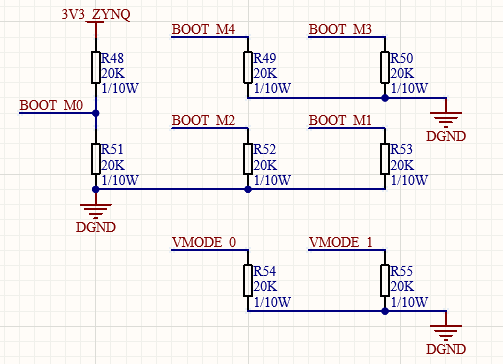
\includegraphics[scale=0.8]{images/bootmode.png}
    \label{fig:boot}
    \fonte{Elaboração própria com base em (UG585, 2023).}
\end{figure}

Por fim, Na Tabela \ref{tab:interfaces}, pode-se verificar qual a função de cada barramento de comunicação, em conformidade com a Figura \ref{fig:arq}. 

\begin{table}[H]
	\ABNTEXfontereduzida
	\caption{\label{tab:interfaces}Descrição das interfaces disponibilizadas.}
	%\begin{tabular}{@{}p{2cm}p{2cm}p{2cm}p{2cm}p{2cm}p{2cm}p{3cm}@{}}
    \centering
    \begin{tabular}{@{} >{\centering}p{4cm} >{\centering}p{8cm} @{}}
    
		\toprule
		\textbf{Interface} & \textbf{Função} \tabularnewline 
        \midrule
         SPI0 & Interface SPI para circuitos internos ao módulo OBDH. \tabularnewline
        \midrule
         SPI1 & Interface SPI para circuitos externos ao módulo OBDH.  \tabularnewline
        \midrule
         QSPI0 & Interface Quad-SPI para memória de inicialização. \tabularnewline
        \midrule
        I2C0  & Interface I2C para circuitos internos ao módulo OBDH. \tabularnewline
        \midrule
        I2C1  & Interface I2C para circuitos externos ao módulo OBDH.  \tabularnewline
        \midrule
        CAN0 & Interface CAN para circuitos externos ao módulo OBDH. \tabularnewline
        \midrule
        CAN1 & Interface CAN para o barramento de expansão. \tabularnewline
        \midrule
         UART0 & Conexão serial para \textit{debugging}. \tabularnewline
        \midrule
         UART1 & Conexão serial para o transceiver RS-485. \tabularnewline
        \midrule
         PS\_GPIO & Sinais de propósito geral de entrada e saída. \tabularnewline

        \bottomrule
	\end{tabular}
	\fonte{Elaboração própria com base na documentação técnica do fabricante.}
\end{table}

Também como mencionado, o projeto terá como memória volátil uma memória do tipo DDR3. Para que se consiga controlá-la, o SoC disponibiliza um banco dedicado para a memória DDR, disposto na  Figura \ref{fig:psddr}. Seus pinos são nomeados conforme (JEDEC, 2008) e suas funções são descritas na Tabela \ref{tab:psddr}. O terceiro banco não é utilizado nesse projeto.

\begin{figure}[H]
    \centering
    \caption{Banco da Memória DDR do PS.}
    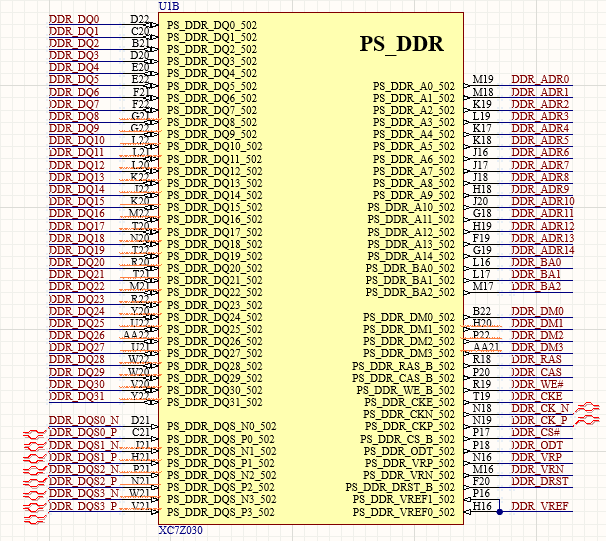
\includegraphics[scale=0.7]{images/psddr.png}
    \label{fig:psddr}
    \fonte{Elaboração própria com base em (UG585, 2023) e (UG933, 2019).}
\end{figure}

\begin{table}[H]
	\ABNTEXfontereduzida
	\caption{\label{tab:psddr}Descrição dos pinos da memória DDR3.}
	%\begin{tabular}{@{}p{2cm}p{2cm}p{2cm}p{2cm}p{2cm}p{2cm}p{3cm}@{}}
    \centering
    \begin{tabular}{@{} >{\centering}p{4cm} >{\centering}p{8cm} @{}}
    
		\toprule
		\textbf{Nome} & \textbf{Descrição} \tabularnewline 
        \midrule
         DDR\_ADRx & Barramento de endereço da memória. \tabularnewline
        \midrule
         DDR\_DQx & Barramento de dados da memória. \tabularnewline
        \midrule
         DDR\_DMx & Sinal da máscara da interface. \tabularnewline
        \midrule
        DDR\_BAx  & Barramento de endereço do banco da memória. \tabularnewline
        \midrule
        DDR\_DQSx  & Sinal diferencial de \textit{Data Strobe}. \tabularnewline
        \midrule
        DDR\_CK & Barramento diferencial do relógio da memória. \tabularnewline
        \midrule
        DDR\_ODT & Sinal de saída de terminação dinâmica. \tabularnewline
        \midrule
        DDR\_CS\# & Sinal de \textit{Chip Select}. \tabularnewline
        \midrule
        DDR\_CKE & Sinal de \textit{enable} do relógio. \tabularnewline
        \midrule
        DDR\_WE\# & Sinal de \textit{Write Enable}. \tabularnewline
        \midrule
        DDR\_CAS & Sinal de endereço da coluna da memória. \tabularnewline
         \midrule
        DDR\_RAS & Sinal de endereço da linha da memória. \tabularnewline
        \midrule
        DDR\_DRST & Sinal de \textit{Reset}. \tabularnewline
        \bottomrule
	\end{tabular}
	\fonte{Elaboração própria com base em (UG585, 2023) e (JEDEC, 2008).}
\end{table}

\subsection{Blocos do PL}

O lado da FPGA do SoC, chamada de PL, é crucial para se ter um hardware versátil. Para isso, tentou-se utilizar a maior parte dos pinos possível, principalmente para o barramento externo. Nesses bancos também se encontram as entradas diferenciais do XADC do SoC. Nas Figuras \ref{fig:plhr} e \ref{fig:plhp} se encontram os esquemáticos dos bancos HR (\textit{High Range}) e HP (\textit{High Performance}), respectivamente. Na Tabela \ref{tab:plzynq}, por sua vez, se encontra a descrição funcional dos pinos por nome.

\begin{figure}[H]
    \centering
    \caption{Banco HR do PL.}
    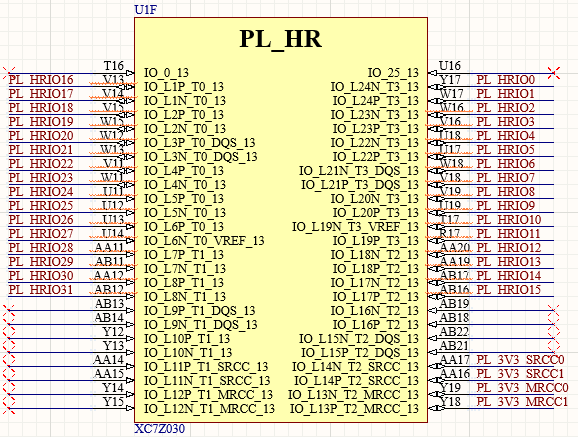
\includegraphics[scale=0.8]{images/plhr.png}
    \label{fig:plhr}
    \fonte{Elaboração própria com base em (UG585, 2023).}
\end{figure}

\begin{figure}[H]
    \centering
    \caption{Banco HP do PL.}
    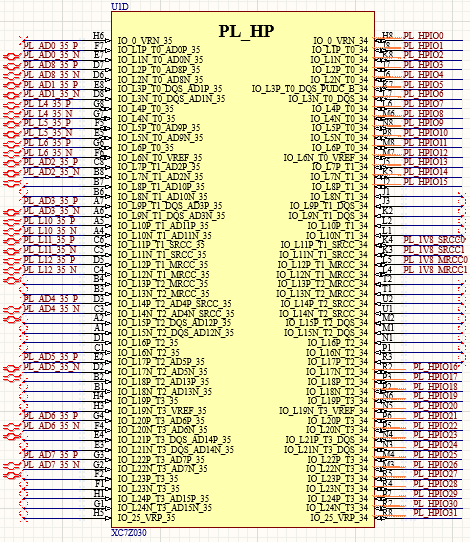
\includegraphics[scale=0.7]{images/plhp.png}
    \label{fig:plhp}
    \fonte{Elaboração própria com base em (UG585, 2023).}
\end{figure}

\begin{table}[H]
	\ABNTEXfontereduzida
	\caption{\label{tab:plzynq}Descrição dos sinais dos bancos do PL.}
	%\begin{tabular}{@{}p{2cm}p{2cm}p{2cm}p{2cm}p{2cm}p{2cm}p{3cm}@{}}
    \centering
    \begin{tabular}{@{} >{\centering}p{4cm} >{\centering}p{8cm} @{}}
    
		\toprule
		\textbf{Nome} & \textbf{Descrição} \tabularnewline 
        \midrule
         PL\_ADx & Entrada diferencial enumerada do XADC. \tabularnewline
        \midrule
         PL\_Lx & Sinal LVDS, presente apenas no banco HP. \tabularnewline
        \midrule
         PL\_HPIOx & Sinal de entrada e saída genérico do banco HP.  \tabularnewline
        \midrule
        PL\_HRIOx  & Sinal de entrada e saída genérico do banco HR. \tabularnewline
        \midrule
        PL\_xx\_SRCCx & Pino capaz de gerar sinal de relógio do tipo \textit{Single Region}. \tabularnewline
        \midrule
        PL\_xx\_MRCCx & Pino capaz de gerar sinal de relógio do tipo \textit{Multi Region}. \tabularnewline
        \bottomrule
	\end{tabular}
	\fonte{Elaboração própria com base em (UG585, 2023).}
\end{table}

\subsection{Pinos de Potência}

Por fim, os pinos de potência devem ser alimentados corretamente. Além disso, é recomendado por (UG933, 2019) que todos os pinos tenham capacitores de desacoplamento o mais perto possível de seus respectivos pinos. Esse circuito e seus capacitores estão dispostos nas Figuras \ref{fig:zpower} e \ref{fig:zcaps}.

\begin{figure}[H]
    \centering
    \caption{Pinos de potência do SoC.}
    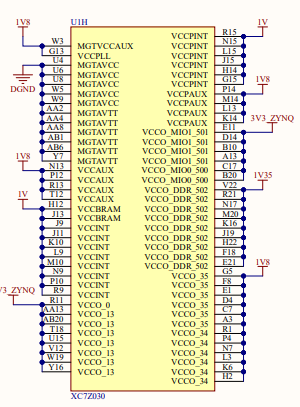
\includegraphics[scale=0.7]{images/zynqpower.png}
    \label{fig:zpower}
    \fonte{Elaboração própria com base em (UG585, 2023) e (UG933, 2019).}
\end{figure}

\begin{figure}[H]
    \centering
    \caption{Capacitores de desacoplamento recomendados.}
    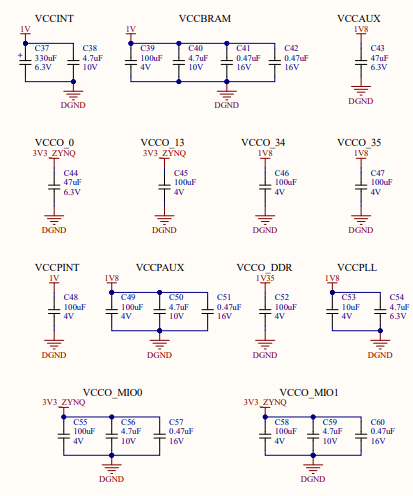
\includegraphics[scale=0.7]{images/zynqcaps.png}
    \label{fig:zcaps}
    \fonte{(UG933, 2019).}
\end{figure}

\section{Memórias}

Nesta seção, abordam-se as principais características das memórias utilizadas no sistema. Serão comentados os circuitos das memórias DDR3L, das memórias Flash NAND e NOR e da memória FRAM.

\subsection{DDR3L} 

A DDR3L selecionada oferece 2 Gb de capacidade de armazenamento, configurada em uma estrutura de 256M x 8 bits. Essa memória opera com tensão reduzida (1.35V), o que a torna eficiente em termos de consumo de energia, crucial para sistemas de satélite. Seu circuito se encontra na Figura \ref{fig:ddr3l}. 

\begin{figure}[H]
    \centering
    \caption{Circuito da memória DDR3L.}
    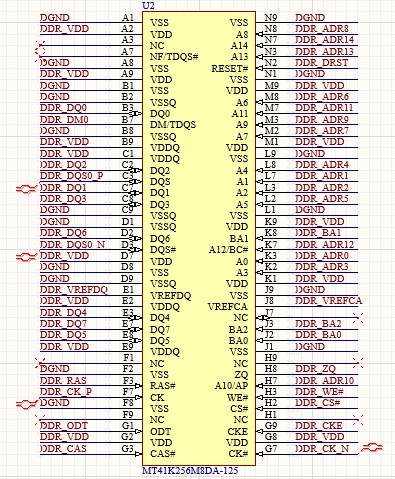
\includegraphics[scale=0.7]{images/ddr3l.png}
    \label{fig:ddr3l}
    \fonte{(MT41K256M8DA-125:K DDR3L Datasheet).}
\end{figure}

\subsection{Flash NOR}

A memória flash NOR, acessada por uma interface QSPI, foi escolhida pela sua capacidade de realizar leituras rápidas, característica que torna esse tipo de memória adequado para armazenamento de firmware ou dados de inicialização do sistema. Seu circuito está presente na Figura \ref{fig:fnor}.

\begin{figure}[H]
    \centering
    \caption{Circuito da memória Flash NOR.}
    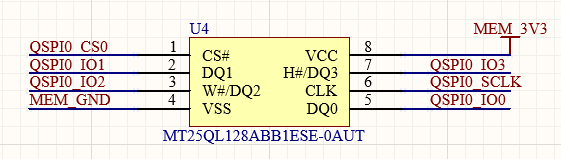
\includegraphics[scale=0.7]{images/flash nor.png}
    \label{fig:fnor}
    \fonte{(MT25QL128ABB1ESE-0AUT Flash NOR Datasheet).}
\end{figure}

\subsection{Flash NAND}

Diferente da flash NOR, a memória flash NAND, acessada via SPI, é utilizada para armazenamento de grandes volumes de dados que não necessitam de acesso frequente, ou seja, dados de uso prolongado, como logs e registros. Seu circuito se encontra na Figura \ref{fig:fnand}.

\begin{figure}[H]
    \centering
    \caption{Circuito da memória Flash NAND.}
    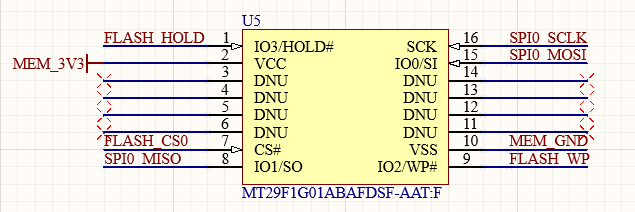
\includegraphics[scale=0.7]{images/flash nand.png}
    \label{fig:fnand}
    \fonte{(MT29F1G01ABAFDSF-AAT:F Flash NAND Datasheet).}
\end{figure}

\subsection{FRAM}

 A FRAM, com acesso por interface SPI, será usada para armazenar dados críticos por sua alta resistência a radiação e alta velocidade de escrita e leitura. Seu circuito se encontra na Figura \ref{fig:fram}.

\begin{figure}[H]
    \centering
    \caption{Circuito da memória FRAM.}
    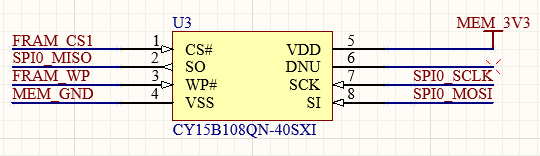
\includegraphics[scale=0.7]{images/fram.png}
    \label{fig:fram}
    \fonte{(CY15B104QN FRAM Datasheet).}
\end{figure}

\section{Periféricos}

Como previsto nos requisitos, são necessários os circuitos do WDT, dos sensores de tensão, corrente e temperatura e do sistema do ADCS. 

Primeiramente, o circuito do WDT, disposto na Figura \ref{fig:wdt}, foi construído para reinicializar o SoC caso o sinal de controle (WDI) não mude por mais de 1,6 segundos (tipicamente). Além disso, o circuito integrado é equipado com um sinal de \textit{reset} manual. 

\begin{figure}[H]
    \centering
    \caption{Circuito do WDT.}
    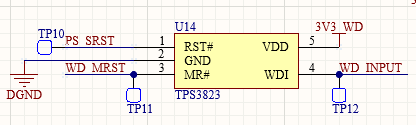
\includegraphics[scale=0.7]{images/wdt.png}
    \label{fig:wdt}
    \fonte{(TPS3823-33QDBVRQ1 Watchdog Timer Datasheet).}
\end{figure}

No circuito do sensor de tensão e temperatura, são monitoradas as tensões de 1 V, 1,8 V, 1,35 V e  0,675 V. Além disso, são medidas as temperaturas tanto do SoC, através dos sinais DXP e DXN, provenientes do diodo interno do Zynq (UG865, 2021), quanto a temperatura da placa, em um transistor externo. O mesmo está disposto na Figura \ref{fig:sense}.

\begin{figure}[H]
    \centering
    \caption{Circuito do monitor de tensão e temperatura.}
    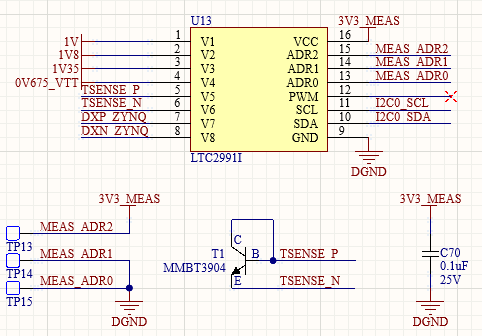
\includegraphics[scale=0.7]{images/sense.png}
    \label{fig:sense}
    \fonte{(LTC2991IMS\#TRPBF Voltage, Current and Temperature Monitor Datasheet).}
\end{figure}

Quanto ao circuito de medição de corrente, foi necessário o cálculo do resistor de medição (Rsense), presente em (6) (INA180A2IDBVR Current Sense Datasheet). Com o valor máximo de Rsense, foi escolhido um resistor menor, de 75 m$\Omega$, para obter uma margem com relação à corrente máxima. Sua saída é lida por uma entrada do XADC do SoC. Seu circuito final está disposto na Figura \ref{fig:csense}.

\begin{equation}
	R_{sense} < Vsp / (G \times Imax) = 1 / (50 \times 2,5) = 80 m\Omega
\end{equation} 

\begin{figure}[H]
    \centering
    \caption{Circuito de medição de corrente.}
    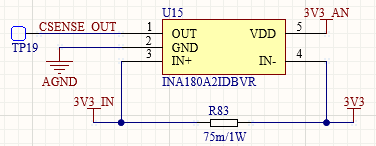
\includegraphics[scale=0.7]{images/current sense.png}
    \label{fig:csense}
    \fonte{(INA180A2IDBVR Current Sense Datasheet).}
\end{figure}

Por fim, o sistema ADCS, controlado pela interface I2C0, será formado pelos circuitos das Figuras \ref{fig:mag} e \ref{fig:gyro}, do magnetômetro e do giroscópio. 

\begin{figure}[H]
    \centering
    \caption{Circuito do magnetômetro.}
    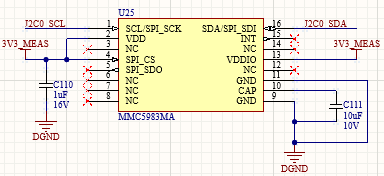
\includegraphics[scale=0.7]{images/magnetometer.png}
    \label{fig:mag}
    \fonte{(MMC5983MA Magnetometer Datasheet).}
\end{figure}

\begin{figure}[H]
    \centering
    \caption{Circuito do giroscópio.}
    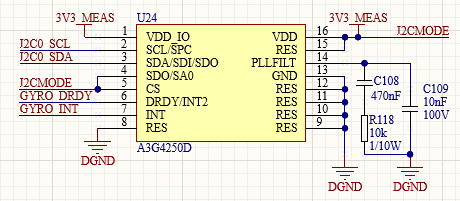
\includegraphics[scale=0.7]{images/gyro.png}
    \label{fig:gyro}
    \fonte{(A3G4250D Gyroscope Datasheet).}
\end{figure}

\section{Conexões entre blocos}

Por fim, todos os blocos foram conectados, usando o princípio de projeto hierárquico fornecido pelo \textit{software} utilizado. A interconexão leva em conta a arquitetura proposta e as necessidades individuais de cada subcircuito apresentado no presente capítulo. Seu esquemático está disposto na Figura \ref{fig:inter}.

\begin{figure}[H]
    \centering
    \caption{Interconexão dos blocos propostos.}
    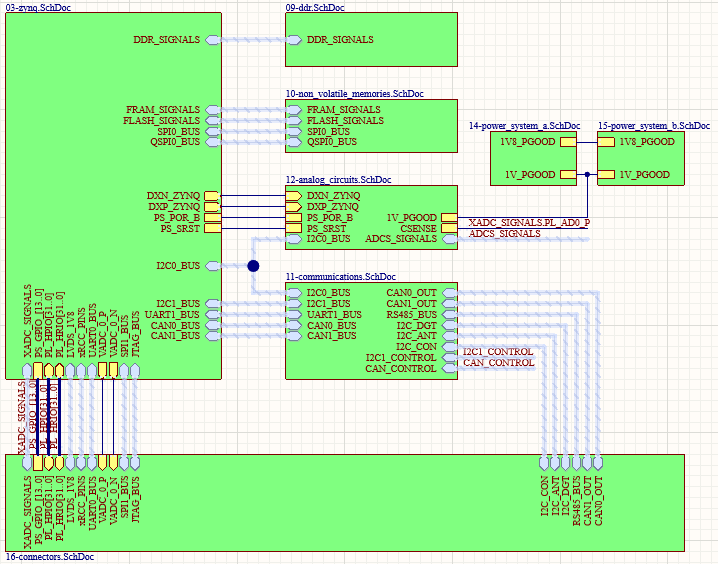
\includegraphics[scale=0.7]{images/conexoes.png}
    \label{fig:inter}
    \fonte{Elaboração própria.}
\end{figure}
